\chapter{Architecture}
\label{arch}

In this section, we present the \name architecture and the underlying protocols in detail. 
Later, we describe our key-establishment system that enables rapid key derivation 
and distribution in large networks. 

\section{\name Bootstrapping}
\label{sec:bootstrapping}

The bootstrapping procedure is performed when a new zone or a new remote site 
(a group of zones along with a \tp) joins the network. 

\paragraph{Zoning Policy} % about zone itself 
A network zone is a logical concept, a group of network segments. A widely adopted 
segmentation technology is Virtual Lan (VLAN) which is used to separate networks on
layer~2. For example, zones are made up of multiple disjoint layer~2 networks
all identified by their corresponding VLAN ID (VID). A VID can be reused as long
as networks using the same VID are kept separate.

In \name, IP subnets correspond to exactly one network zone, such that the zone
a host belongs to can be identified by the host IP address. The same private
address spaces can be a part of different zones, and they are distinguishable by a
combination of their ASN (autonomous system number) and IP subnet. 
% \ml{Where does the ASN come from here? Couldn't the same private address space be used on different sites which are located in the same AS?} 
Consequently, each zone is defined as:
\noindent 
\begin{subequations}
\begin{align}
ASN \times IPsubnet & \mapsto VID, \\
\tp \times VID & \mapsto zoneID.
\end{align}
\label{eq:zoning}
\end{subequations}
\noindent 
% \claude{VID $\subseteq$ \{ASN: IPsubnet\}}
% \claude{ZoneID $\subseteq$ \{TP : VID\}}
% \claude{I was again thinking about this notation. I feel like the element notation conveys the wrong idea that one VID/ZoneID is limited to exactly one ASN:IP or TP:VID respectively. Maybe the subset ($\subseteq$) relation is more suitable here.}
% \ml{Is the VID supposed to actually \emph{consist} of ASN and IPSubnet (in terms of the bit representation) or rather \emph{refer} to (a set of) ASN:IPSubnets? In the latter case, a relation or function from VIDs to the combination of ASN:IPSubnets might be the most appropriate notation (same holds for ZoneIDs).}
% \ml{When typesetting names in math mode it is preferred to sourround them by ``mathit'' or ``text'' (whichever is preferred), as otherwise individual letters are understood as individual variables and spacing is suboptimal.}
The way zones are described here corresponds to how enterprises typically
segment their networks today, upholding backward compatibility and consequently
deployability. Furthermore, \name does not depend on the specific layer~2 protocols used 
at each site. 

Every zone is under one ownership, e.g., company A. In case multiple companies
want to collaborate by sharing certain network zones, it is one company that 
creates and owns the zones and the other companies simply join the network.

\paragraph{Zone Transfer Policy}
To allow network operators to explicitly express their zone transfer policies, we 
consider both denylist and allowlist-based policy establishment. 
% \ml{There are currently some suggestions of replacing blacklist/whitelist by \{block,deny\}list/allowlist.} 
This is a
mature approach commonly used in modern network management systems, enabling flexible
and agile orchestration of complex networking policies. The following depicts the
zone transfer policy format:
\noindent 
\begin{equation}
<zone_{dst}, zone_{src}> \\ 
\Rightarrow~<action, priority, time>
\label{eq:policy}
\end{equation}
\noindent 
$action$ determines the corresponding action for the given source and destination
zone pair, e.g., \texttt{forwarding}, \texttt{drop}, and \texttt{established}. Similar
to \textit{iptables} rules, \texttt{forwarding} would allow any incoming packets from
the source zone whereas \texttt{drop} discards all traffic. \texttt{established} allows
incoming traffic for all established connections. 

In an event of conflict where $zone_{src}$ has different
access authorizations for the $zone_{dst}$, the conflict can be resolved by the field 
of $priority$. That is, a policy with a higher priority would be enforced in the zone 
If conflicting policies have the same priority, the most recently established policy 
according to $time$ would be enforced.

% In principle, VLAN is an layer~2 technology, running on a local network. To allow
% such VLANs 

\paragraph{Translation Point Initialization} % about tp
A \tp is initialized when a new remote site opens, prior to any communication between
zones. The initialization process has mainly two goals: i) bootstrap a secure channel 
with its controller to exchange control-plane messages, and ii) establish secure tunnels 
with other \tps for data transmission.
% A \tp is initialized when a new remote site opens, prior to any communication between
% zones. The initialization process has mainly three goals: i) bootstrap a secure channel 
% with its controller to exchange control-plane messages, ii) synchronize with the controller
% in terms of zone creation and translation policies, and iii) establish secure tunnels with
% other \tps for data transmission.

Upon bootstrap, a \tp performs a \textit{client-authenticated TLS handshake} with its 
controller in order to exchange their certificate, and agree on a cipher suite and compression
method. The \tp finds the corresponding address in its configuration file. This means 
that, prior to first use, there needs to be an out-of-band setup where the \tp is 
configured. This can either be done by the owner of the controller shipping a pre-configured 
machine to the new remote location or by the remote location setting up a machine and 
granting the controller owner management access to the given machine. Bootstraping \tps 
with multiple controllers will be described in~\S\ref{sec:distributedcontroller} with
practical considerations such as controller discovery, \tp migration, and policy consistency.

The controller synchronizes with \tps to keep their list of other \tps in the network 
up-to-date. To this end, the controller frequently pushes a list of relevant \tps with 
which a \tp can communicate.
% \claude{actually only the relevant subset of \tps is needed} 
% \jk{How does controller know the "relevant" \tps?}. 
This can be done either regularly (e.g., on a daily basis) or occasionally
(e.g., when a new \tp joins the network).
\tps then establish a secure channel with new \tps. To prevent \tps from using a stale \tp list,
the shared \tp list is associated with a time to live (TTL) value. 
% \claude{what does behind mean here? Still confused by this point? Does it mean in order to prevent TPs which were left behind by the synchronization from trying to fetch keys from stale TPs we associate the list with a timeout? }

For ``\textit{trust-even-before-first-use}'', 
% \ml{to me, this term refers to implicitly trusting the communication partner at first use. This is not what is used here where the entities explicitly authenticate each other.} 
the \tps and controller must be able to verify each 
other, preventing: i) a legitimate controller pushing information to an unauthorized \tp, 
and ii) a legitimate \tp connecting to a bogus controller or \tp under an attacker's control.
We ensure source authenticity of the \name entities by leveraging PKI-based identities.
The main idea behind the source authenticity is that all the \tps and controllers obtain
digital certificates for their IP address from a public key infrastructure (PKI). The owner 
of the entities (e.g., an enterprise) is a certificate authority, and issues the certificates
before an entity bootstraps. To this end, we consider well-established practices, e.g.,
the Resource Public Key Infrastructure (RPKI)~\cite{rfc7115,rfc6810}.
%  in the current Internet 
% or the SCION control-plane PKI in SCION future Internet architecture~\cite{Perrig2017}.
% \ml{At this point it is unclear what this has to do with SCION.}

% Upon bootstrapping, a \tp perform the \textit{client-authenticated TLS handshake} with its
% controller. That is, the \tp and controller exchange their certificate, agree on a cipher
% suite and compression method. Once the secure channel establishes, the \tp sends the 
% controller a \texttt{ZoneSync} request as:

% \begin{equation*}
% TP \rightarrow C: \Rightarrow~<action, priority, time>.
% \end{equation*}


\section{Protocol Description}
\label{sec:protocol}

Now, we describe how two end hosts within different remote sites are able to communicate. 
Figure~\ref{fig:protocol} illustrates a protocol level design including authorization,
forwarding, and verification. A detailed header design follows.

\begin{figure}[t]
\begin{center}
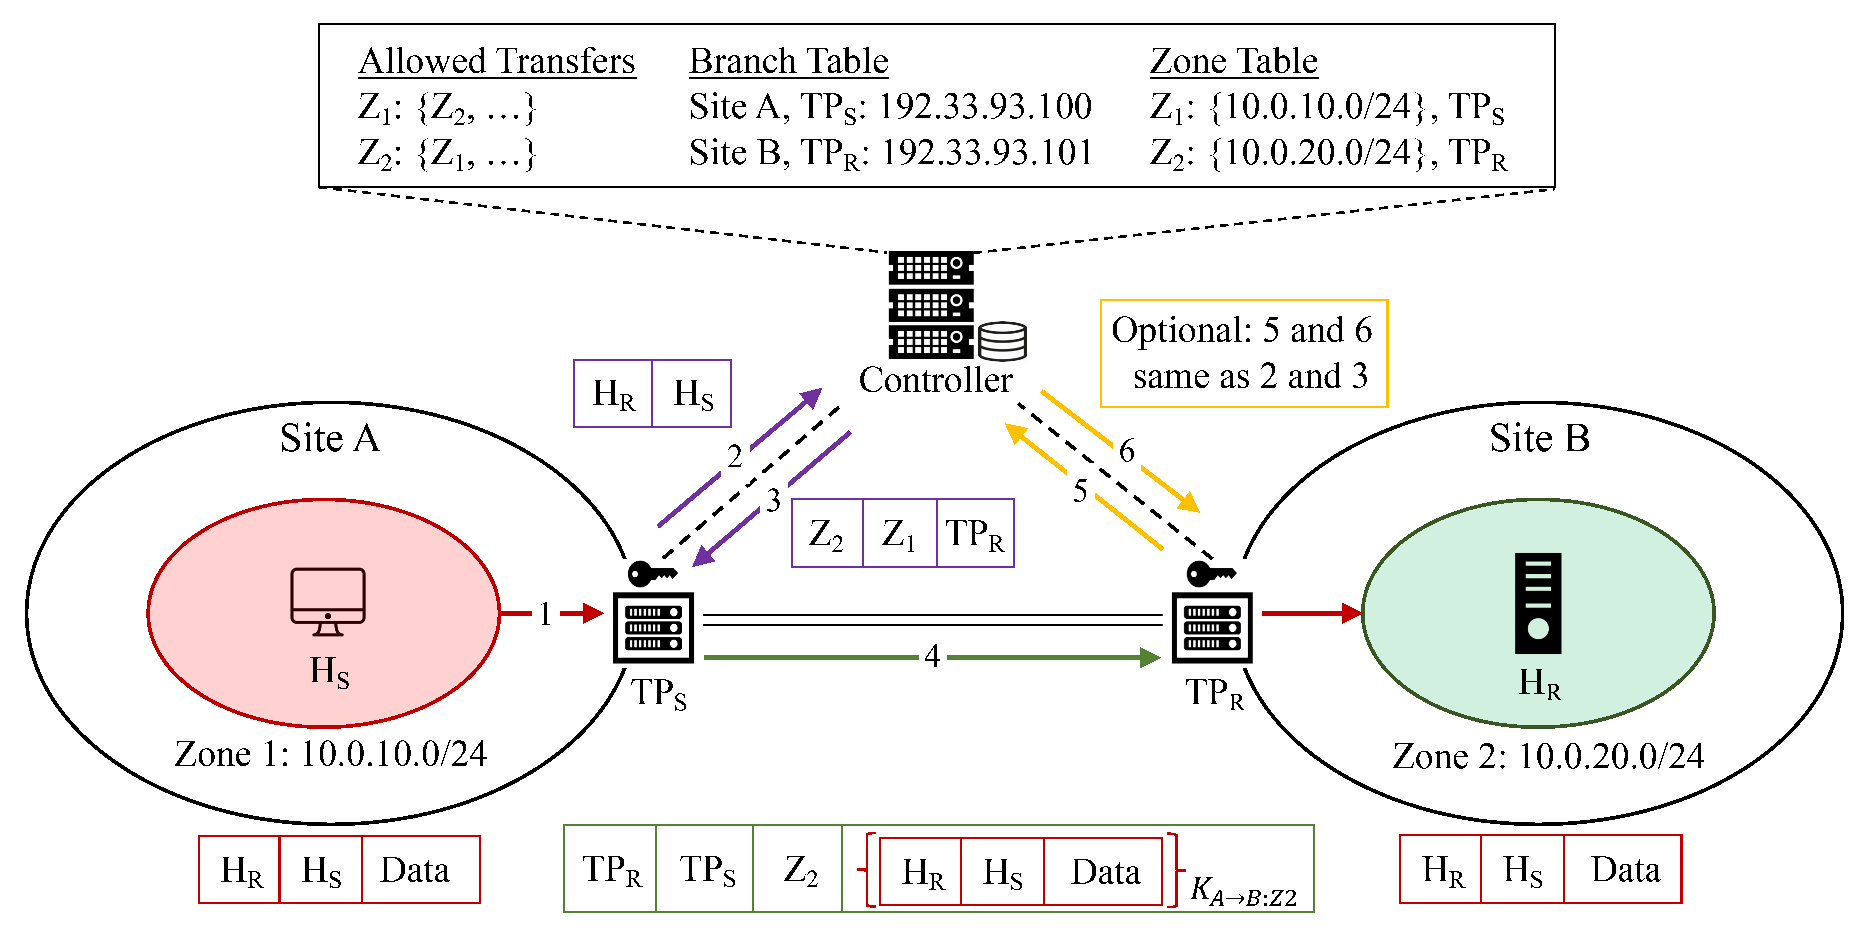
\includegraphics[width=.9\textwidth]{protocol.eps}
\end{center}
\caption{Protocol details for data forwarding. The controller frequently updates \tps 
with the latest zone transfer policies.}

\label{fig:protocol}
\end{figure}

% \paragraph{Zone Migration}

\paragraph{Zone Transfer Authorization}
End hosts behind a \tp operate as they normally would when they reside in a local network connected to a commodity gateway. That is, without any acknowledgment on network changes, a sender $H_S$ 
sends a packet to the receiver $H_R$. If $H_S$ and $H_R$ are residents of the same subnet 
(namely the same zone), the packet will be directly steered to the destination by the local 
forwarding devices. If $H_R$ is in a different subnet (or a remote site) however, the packet
is first delivered to $\tp_S$ since $\tp_S$ is the gateway of $H_S$. % (\tcircled{1}). 

To determine if the packet is allowed to be forwarded to the given destination zone $B$, $\tp_S$
needs an explicit zone-transfer policy for the given source and destination pair. Ideally, 
the policy is cached in the $\tp_S$'s zone transfer table. In case the cache misses, $\tp_S$ 
acquires the policy from the controller $C$ as follows:

\begin{enumerate}
	\item $\tp_S$ requests a zone-transfer policy from $C$:
	\begin{equation}
		\tp_S \rightarrow C : H_R~|~H_S
	\label{eq:authreq}
	\end{equation}
	\item $C$ replies with the zone-transfer policy:
	\begin{equation}
		C \rightarrow \tp_S : \\
		Z_R~|~Z_S~|~rule~|~\tp_R~|~ExpTime
	\label{eq:authrep}
	\end{equation}
\end{enumerate}

The controller consults the zone-transfer policy to see if the packet is allowed to be forwarded
to $H_R$, more specifically to destination zone $Z_B$. To this end, the controller 
first checks the corresponding zone information (Equation~\ref{eq:zoning}), and matches 
it with the zone transfer rules (Equation~\ref{eq:policy}). The authorization result is
then delivered to the requesting \tp along with the corresponding source and destination 
zone identifiers ($Z_R$ and $Z_S$ respectively), the destination \tp address 
($\tp_R$), and the expiration time ($ExpTime$) for the policy. $ExpTime$ can be an arbitrary
number, but we consider it to be a small number used for policy freshness.

\paragraph{Data Forwarding}
The \tp discards the packet (Host Unreachable) if $rule=$ \texttt{drop}. Otherwise, 
the \tp looks up its routing table and transmits the packet. There exist two types of 
zone transfer cases: one for local (same-site) zone transfers and another for remote zone 
transfers as addressed in \S\ref{sec:casestudy}. For the local zone transfer, the \tp 
simply rewrites the Ethernet header by following the local layer~2 protocol, and 
forwards it through a corresponding interface. Since the local network is assumed to
be trustworthy, no additional packet processing is necessary apart from the authorization.

For the remote zone transfer, the \tp is responsible for the secure transmission of the
packet towards the destination \tp. Recall that it is important for the inter-domain 
zone transfer packet to keep confidentiality and integrity in transmission. We therefore 
leverage the notion of secure tunneling, i.e., the IPSec tunnel mode~\cite{rfc4301,rfc4303}, 
meaning that the original packet is wrapped, encrypted, authenticated, and attached to a 
new IP header. The new packet layout is formed as follows:
\noindent 
\begin{subequations}
\begin{align}
EIP & = \{H_R~|~H_S~|~payload\}_K, \\
AT & = MAC_K(Z_R~|~EIP), \\
\tp_S \rightarrow \tp_R &: \tp_R~|~\tp_S~|~Z_R~|~AT~|~EIP.
\end{align}%
\label{eq:forwarding}%
\end{subequations}%
The given field name, Encrypted original IP payload (EIP), is self-explanatory. 
% \ml{I'm not familiar with ``EIP'', is this a well-known concept?} 
The original 
packet including IP header and payload is encrypted with a secret key $K$ pre-shared 
between $\tp_S$ and $\tp_R$. By encrypting the original packet and encapsulating it into
the new IP datagram, we ensure confidentiality on the original payload as well as the 
host identities. We also introduce an Authentication Token (AT) which is placed in front of 
the EIP and contains a message authentication code (MAC) covering EIP and the destination 
zone identifiers.
AT provides integrity over the entire packet except the outer IP header field which could 
be modified in transit.
% \ml{Maybe this detailed description is not really necessary as IPSec is well established.}

% \ml{I'm a little confused by the previous and next paragraph: Do you now use an existing IPsec protocol or create your custom IPsec-like tunnel?}

The main difference to the Encapsulating Security Payload (ESP) on IPSec tunnel mode 
is that, rather than having site-to-site symmetric keys, we use site-zone pairwise keys.
That is, the keys used for every triplet of \{$\tp_{src}~|~\tp_{dst}~|~zoneID_{dst}$\} 
differs, providing a variety of unique symmetric keys even for the same pair of \tps. 
% \ml{Wouldn't that be possible with plain IPsec as well?}
In addition, by conveying only $zoneID_{dst}$ in the header, zone pair information, which 
could lead to the potential disclosure of the zone structure
and their transfer rules, is not exposed. 


% The site-zone specific key binding gives us the following 
% advantages; i) a variety of symmetric keys for the same pair of \tps, and ii) an ability 
% of zone transfer verification at the tunnel endpoint. In a nutshell, it provides
% achieving a higher forwarding secrecy. 

% an outer IP header indicating two tunnel endpoints. 


\paragraph{Verification}
% full verification: authentication check + zone transfer policy check
The destination \tp performs two steps of verification upon packet arrival: authentication
and authorization. By extracting the quartet information from 
the header, $\tp_R$ first derives the corresponding symmetric key and recalculates AT to
see whether the MAC matches the original AT value. This step is used to verify packet
integrity as well as authenticity since only the two parties can derive the same 
symmetric key. If the match fails, it means that either the packet integrity is compromised
or source authentication failed. Therefore, the packet is discarded.

To further verify authorization, $\tp_R$ obtains $H_S$ and $H_R$ by decrypting EIP, and 
verifies if $H_S$ is authorized for the zone transfer towards $H_R$. Similar to $\tp_S$,
$\tp_R$ might send a request to its controller to acquire the authorization policy when
the policy is missing in its database (Equations~\ref{eq:authreq} and~\ref{eq:authrep}). 

% half verification (trusted TP model): authentication check only
In principle, \name is constructed under a single administrative domain such that all the 
core entities, i.e., \tps and controllers, are trustworthy. One of the main advantages of 
this trust model is that the authorization check performed by the sender side \tp is also 
trusted. The receiver-side \tp therefore does not necessarily verify the zone transfer 
authorization. Upon receiving a packet, $\tp_{dst}$ checks the authenticity of the packet, 
decrypts EIP, and forwards the original IP packet to the destination host. This trust
model could simplify the entire verification process significantly by omitting the
authorization step which requires an additional challenge-response protocol to the 
controller, improving practicality for \tps running at small branches limited in 
operational resources. 

\section{Key Management}
\label{sec:keymanagement}

In order for the \tps to create and verify authenticators based on symmetric cryptography 
we need a scheme to distribute keys amongst them. Ideally, the keys used for every 
triplet of \{$\tp_{src}~|~\tp_{dst}~|~zoneID_{dst}$\} should be different. Additionally, 
ease of key management is a major concern as key distribution mechanisms in today's 
Internet, such as IPsec~\cite{rfc2408,rfc2409,rfc4306}, are complicated and introduce 
management overhead. To alleviate these problems we propose a key management system 
based on a state-of-art key management system called PISKES \cite{rot2020piskes}.

% descrive major differences from PISKES
Major modifications to PISKES introduced for \name key management stem from the following requirements: first,
in the context of network zoning, we require a high degree of confidentiality on top of
authenticity to protect sensitive information. PISKES mainly targets authenticity for 
network entities, not confidentiality. Second, \name does not trust ASes hosting zones
for enterprises. PISKES's key establishment relies on the asymmetric key pair issued by
each AS, that might cause a \textit{man-in-the-middle} (MITM) vulnerability. Furthermore, it is unlikely that an AS 
wants to have a dedicated key-establishment service for each enterprise, which would require 
additional management overheads and deployments amongst ASes. Third, \name requires key 
management at zone granularity, while PISKES is intended to support key exchanges at a 
higher granularity (e.g., per host or application). Thus, there is a design headroom which 
could simplify the architecture, reducing functional complexity and enhancing management
scalability.

Driven by this, we redesign the PISKES's key-derivation architecture removing the
AS dependency (i.e., the AS keys and the dedicated key servers at each AS), meaning
that an enterprise has full control over distributed network zones and does not
need to trust other ASes for inter-zone networking. Additionally, we simplify the key 
design to work at zone granularity, supporting faster key-derivation while
providing the same level of security. 

\paragraph{Key Hierarchy}
PISKES introduces a key hierarchy that allows services to dynamically derive symmetric 
keys in a fast and easy manner. We adapt the concept to support key derivation in the 
context of network zoning. The key hierarchy is as follows:

\begin{itemize}
	\item 0th-level key: $S_{\tp}$ is the secret value generated by each \tp individually.
	\item 1st-level key: a \tp derives different symmetric keys for other \tps from the
	local secret value $S_{\tp}$. The derived symmetric keys are called first-level keys and 
	are calculated as
	\begin{equation}
		K_{A \rightarrow B} = PRF_{S_{{TP}_B}}(A),
		\label{eq:1stkey}
	\end{equation}
	where $B$ stands for the receiving \tp address and $PRF$ is a secure pseudo-random 
	function. Since only one of the two parties can derive this key, it is necessary for 
	the other party, in this case $A$, to fetch the shared symmetric key by contacting 
	$B$. We note that, in contrast to PISKES, the arrow direction
	in the notation indicates the communication direction for which the key is used.
	% \ml{Maybe mention that this is reversed compared to the PISKES paper?}
	% \claude{here,  should be sending TP, not the receiver}
	% \jk{I don't like the current notation. It's so confusing. Let's discuss again.}
	% % The key exchange is authenticated and encrypted using TLS with the certificates 
	% issued to every \tp.
	\item 2nd-level key: from the first-level keys, second-level keys are derived to
	provide diverse symmetric keys for each zone within the same source and destination 
	\tp pairs. The second-level keys are calculated as
	\begin{equation}
		K_{A \rightarrow B:Z} = PRF_{K_{A \rightarrow B}}(Z).
		\label{eq:2ndkey}
	\end{equation}
	$Z$ is the zone ID of the target zone where the destination host resides. 
\end{itemize}

% \ml{Maybe use 1st/first, 2nd/second consistently?}
This hierarchical key structure benefits us in multiple aspects: first, it delivers
key diversity. Since a second-level key is bound to a destined zone, it enables 
each zone to have different keys even for the same pair of source and destination \tps. 
Second, it is easy for \tps to efficiently derive the symmetric keys as all the
required inputs to build the same keys (i.e., local and remote \tp address, and 
destination zone) are contained in the packet header. In particular, a remote \tp 
thus can derive the key directly from the packet header without a memory lookup. 
% \claude{this is only true for the receiving party}
Finally, since all second-level keys are derived directly from first-level keys, 
the system scales linearly with the number of \tps, not the number of zones, achieving scalability.

\paragraph{Bootstrapping Keys}
Each \tp randomly generates a local secret value $S_{\tp}$, the root of the \tp-specific 
key hierarchy. Since the first and second-level keys are derived from the secret value 
recursively, they inherit the randomness and secrecy of $S_{\tp}$. Driven by this, we 
consider a non-deterministic random number generator. The randomly generated secret value 
never leaves \tp premises and is frequently renewed, e.g., on a daily basis, to achieve 
perfect forward secrecy~\cite{rfc1363}.


% Each \tp randomly generates a local secret value $S_{\tp}$. Since the secret value is 
% the root of the \tp-specific key hierarchy, it never leaves the \tp premises and is 
% frequently renewed, e.g., daily basis. For a true randomness of the key generation,
% it is possible to consider 

% Since the 1st and 2nd-level keys are derived from the secret value, they inherit the
% randomness of $S_{\tp}$. For a true randomness of the key derivation, applying an
% nondeterministic random number generator (e.g., quantum random number generator) seems
% ideal. Nevertheless, we

\paragraph{Key Establishment}
% first-level key
Key establishment precedes first data transmission. To establish a first-level key, 
the source \tp initializes the key exchange protocol by sending a key exchange request:
\noindent 
\begin{subequations}
\begin{align}
req & = A~|~B~|~ValTime, \\
\tp_A \rightarrow \tp_B & : req~|~\{req\}_{K^-_A},
\end{align}
\label{eq:req}
\end{subequations}
% \begin{equation}
% 	Req_{A \rightarrow B} = \{A | B | ExpTime\}_{K^-_A},
% \end{equation}
\noindent 
where $ValTime$ represents the validity period of the request. The request is signed with
the requesting \tp's private key ${K^-_A}$, meaning that the receiving \tp can verify the
authenticity of the request packet. Recall that, for authenticity of \name entities, each
\tp certifies own public/private key pair with a certificate issued by the trusted CA,
e.g., the owner of the network zones.

Upon receiving the key exchange request, $\tp_B$ verifies the source authenticity and 
checks the validity of $ValTime$. If the request is valid $\tp_B$ derives a 
first-level key from the local secret value $S_{{\tp}_B}$ and replies back to the requester.
The reply packet is formed as follows: 
\noindent 
\begin{subequations}
\begin{align}
K_{A \rightarrow B} & = PRF_{S_{{\tp}_B}}(A), \\
rep & = \{B~|~K_{A \rightarrow B}~|~ExpTime\}_{K^+_A}, \\
\tp_B \rightarrow \tp_A & : rep~|~\{rep\}_{K^-_B},
\label{eq:rep}
\end{align}
\end{subequations}
\noindent 
where $ExpTime$ denotes the expiration time of the first-level key, $K^+_A$ is the 
$\tp_A$'s public key used for encryption, and $K^-_B$ is the $\tp_B$'s private key to 
sign the reply packet. Finally, the requesting \tp verifies the validity of the reply
packet and caches $K_{A \rightarrow B}$ until it expires. 
% Note that, the expiration 
% time inherits the lifetime of the local secret value since the key issuer $\tp_B$ 
% dynamically derives the same first-level key on fly from its local secret, not caching 
% it unlike sender \tps, enabling fast verification for incoming traffic without a memory 
% lookup. To be able to derive the correct first-level keys, all the first-level keys are 
% therefore reissued when the local secret value is renewed.
Note that the key exchange
protocol could be replaced with well-established key exchange protocols, such as IKE 
\cite{rfc7296}.

Ideally, a \tp prefetches all the first-level keys for other \tps it wishes to communicate 
with. The \tp acquires the list of active \tps from its controller and initiates the key 
exchange protocol for these \tps in advance. This is feasible because the number of \tps for
an enterprise is surely limited; for example, the total number of branches that the Bank of America has in 2019 is approximately 4.6k~\cite{statista2019boa}. 
Each branch would need just one \tp, which means that a \tp needs
to prefetch 4.6k first-level keys. Nonetheless, on-demand key fetching is also possible. 
In particular, when the current first-level key expires in the middle of on-going data
transmission or a new \tp joins, a key exchange can be initiated.

% second-level key
\tps are also responsible for second-level key establishment. However, this does not 
require any key exchange protocol. Upon data transmission, source and destination \tps 
are able to dynamically derive the same second-level key for the destined zone from the
shared first-level key as shown in Equation~\ref{eq:2ndkey}.


% since the second-level keys are directly derived from the shared first-level key


% \paragraph{Key Expiration}

% \subsection{Zone Transfer Policy}
